% Source: tex/chapters/ch06/01_全体概要：この章で学ぶこと.tex
\subsection*{全体概要：この章で学ぶこと}
\addcontentsline{toc}{subsection}{全体概要：この章で学ぶこと}

この章は、ソフトウェアを本番環境で安定して動かし続けるための知識領域を扱う。運用は、開発が終わった後に突然始まる作業ではない。新しいソフトウェアを作る意思決定が行われた時点から、運用計画、保守計画、サービス水準、容量、障害時の復旧、セキュリティ、監視、自動化を考え始める必要がある。

\begin{pointbox}{到達目標}
この章を読み終えると、次のことができるようになる。
\begin{itemize}
  \item ソフトウェアエンジニアリング運用の範囲を説明できる。
  \item 運用計画、運用提供、運用制御の三つのプロセス群を区別できる。
  \item 配備とリリース、インシデントと問題、バックアップとフェイルオーバーの違いを説明できる。
  \item 可用性、継続性、サービス水準、容量、リスク管理の関係を説明できる。
  \item DevOps、IaC、SRE、継続的デリバリー、自動テスト、監視とテレメトリが運用にどう関係するかを説明できる。
\end{itemize}
\end{pointbox}

\begin{figure}[htbp]
\centering
\IfFileExists{assets/generated_figures/ch06/fig-ch06-01.png}{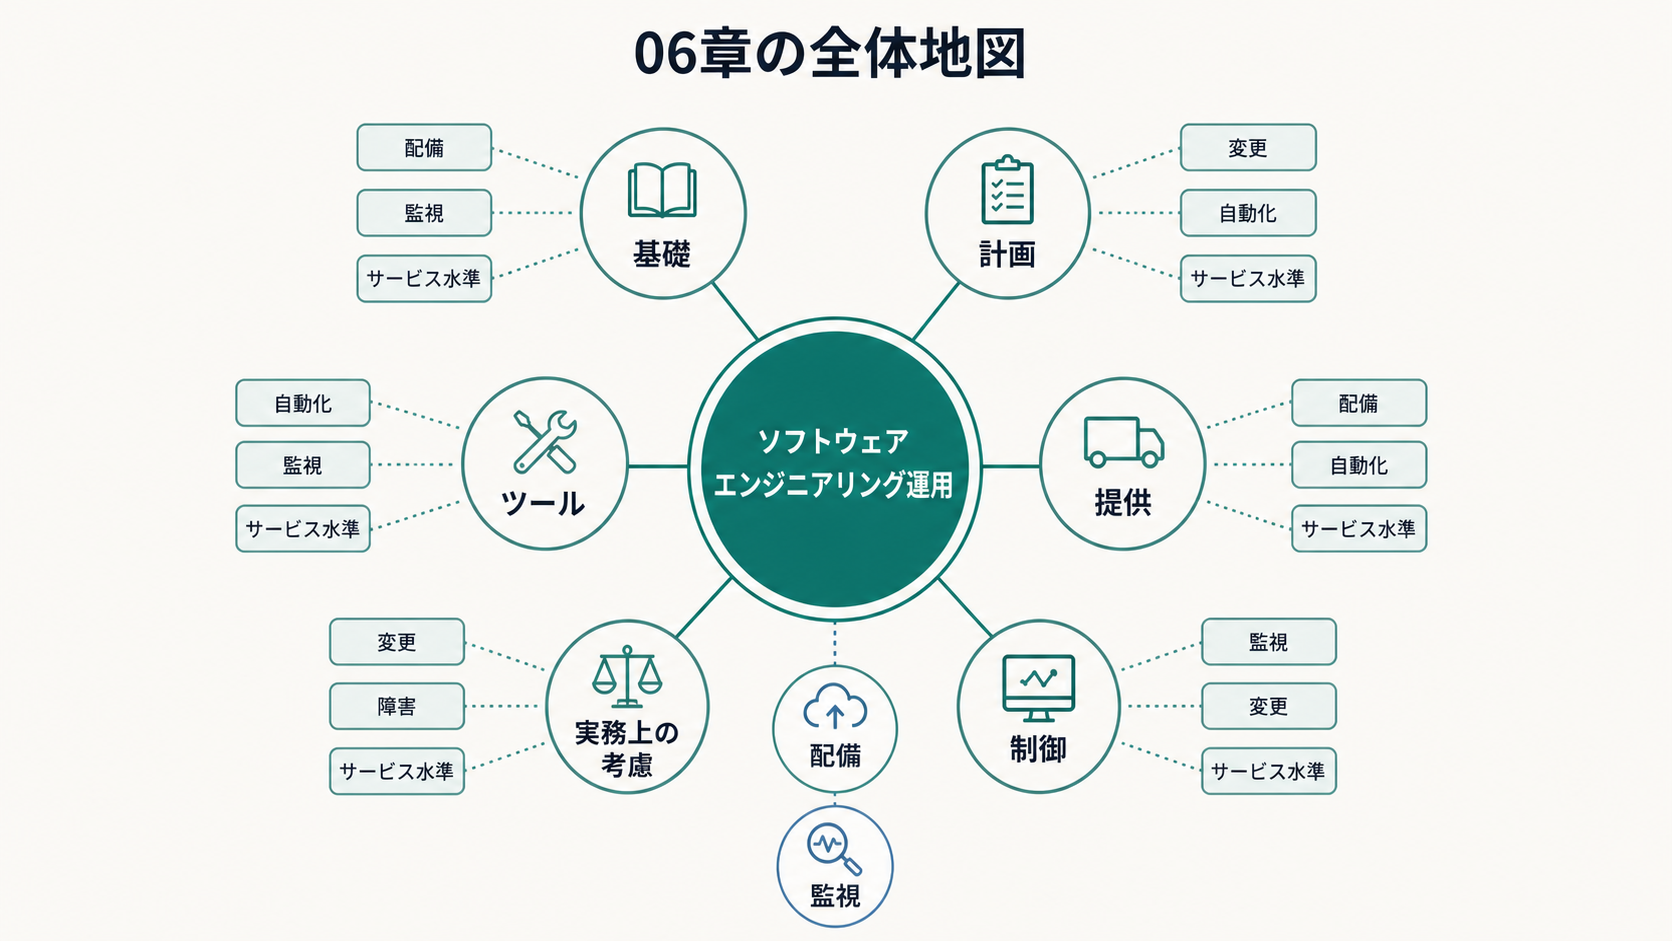
\includegraphics[width=0.96\linewidth]{assets/generated_figures/ch06/fig-ch06-01.png}}{\fbox{\parbox[c][48mm][c]{0.9\linewidth}{\centering 画像生成待ち\\06章の全体地図}}}
\caption{06章の全体地図}
\label{fig:ch06-01}
\end{figure}
